\section{Discovered objects}

Below we list some of the variable objects that have discovered as a result of running the automated pipeline on a fraction of the ULTRACAM archive. The pipeline is usually invoked by running a single command on a night's worth of data. For example, to build the light-curves for the night of, say, emph{2014-08-21}, then a single command, emph{daybuilder.py 2014-08-21} is issued from the command line. The pipeline then runs through all of the data for that night and generates a set of web pages. Depending on the amount of data for that night, this can take 1 hour to 8 hours. 

\subsection{Object identification}
For each night, an 'index page' is generated, which shows a list of all of the runs in the night along with thumbnail images of the field of view. This allows the user to quickly navigate to the runs that are 'of interest'. In other words, runs that contain science data, rather than acquisitions, biases, flat-fields. By clicking on the thumbnail of the run, they are taken to a 'run page'. This page shows the full image for each of the three channels. These images are created by stacking all of the individual frames in the run. The page also shows all of the objects that have been identified and have light-curves available. The user can view the light-curves by using the mouse to click on each object, or can scroll through all of the light-curves systematically, by using the left and right arrow keys. 

Scrolling through the light curves in a systematic fashion makes it easy for the user to quickly identify which objects are showing an obvious variability. All of the objects listed below were discovered in this way. 

The task is made relatively easy in the browser interface and it is possible to inspect the light curves at a rate of about 1-2 objects per second. In future, we plan to apply some statistical tests to the data to perform the light curve inspection as a stage of the automated pipeline. Algorithms to perform these sorts of tests are already known and becoming increasingly more widespread as more large scale sky surveys are being used throughout astronomy research. We plan to re-use work from one or more of these surveys. References to VVV, LSST, NGTS, Wasp, Astrokit software, etc.

\subsection{Eclipsing binaries}

  \begin{tabular}{l l}
  Classification & W Uma contact binary \\
  ObjectID & 2013-07-21-run010-48 \\
  RA, DEC & 19:44:09/8, 40:16:34.4 (J2000) \\
  Run date & 2013-07-21 \\
  Pixel position & (452, 332) \\
  URL: & \small \url{http://deneb.astro.warwick.ac.uk/phrnaw/sitedev/2013-07-21/run010.html} \\
  Finding chart & 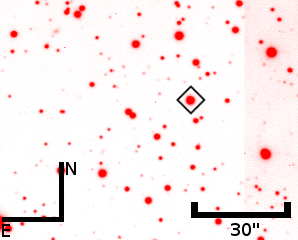
\includegraphics[width=60mm]{images/2013-07-21-run010-48.png} \\
  \end{tabular}
  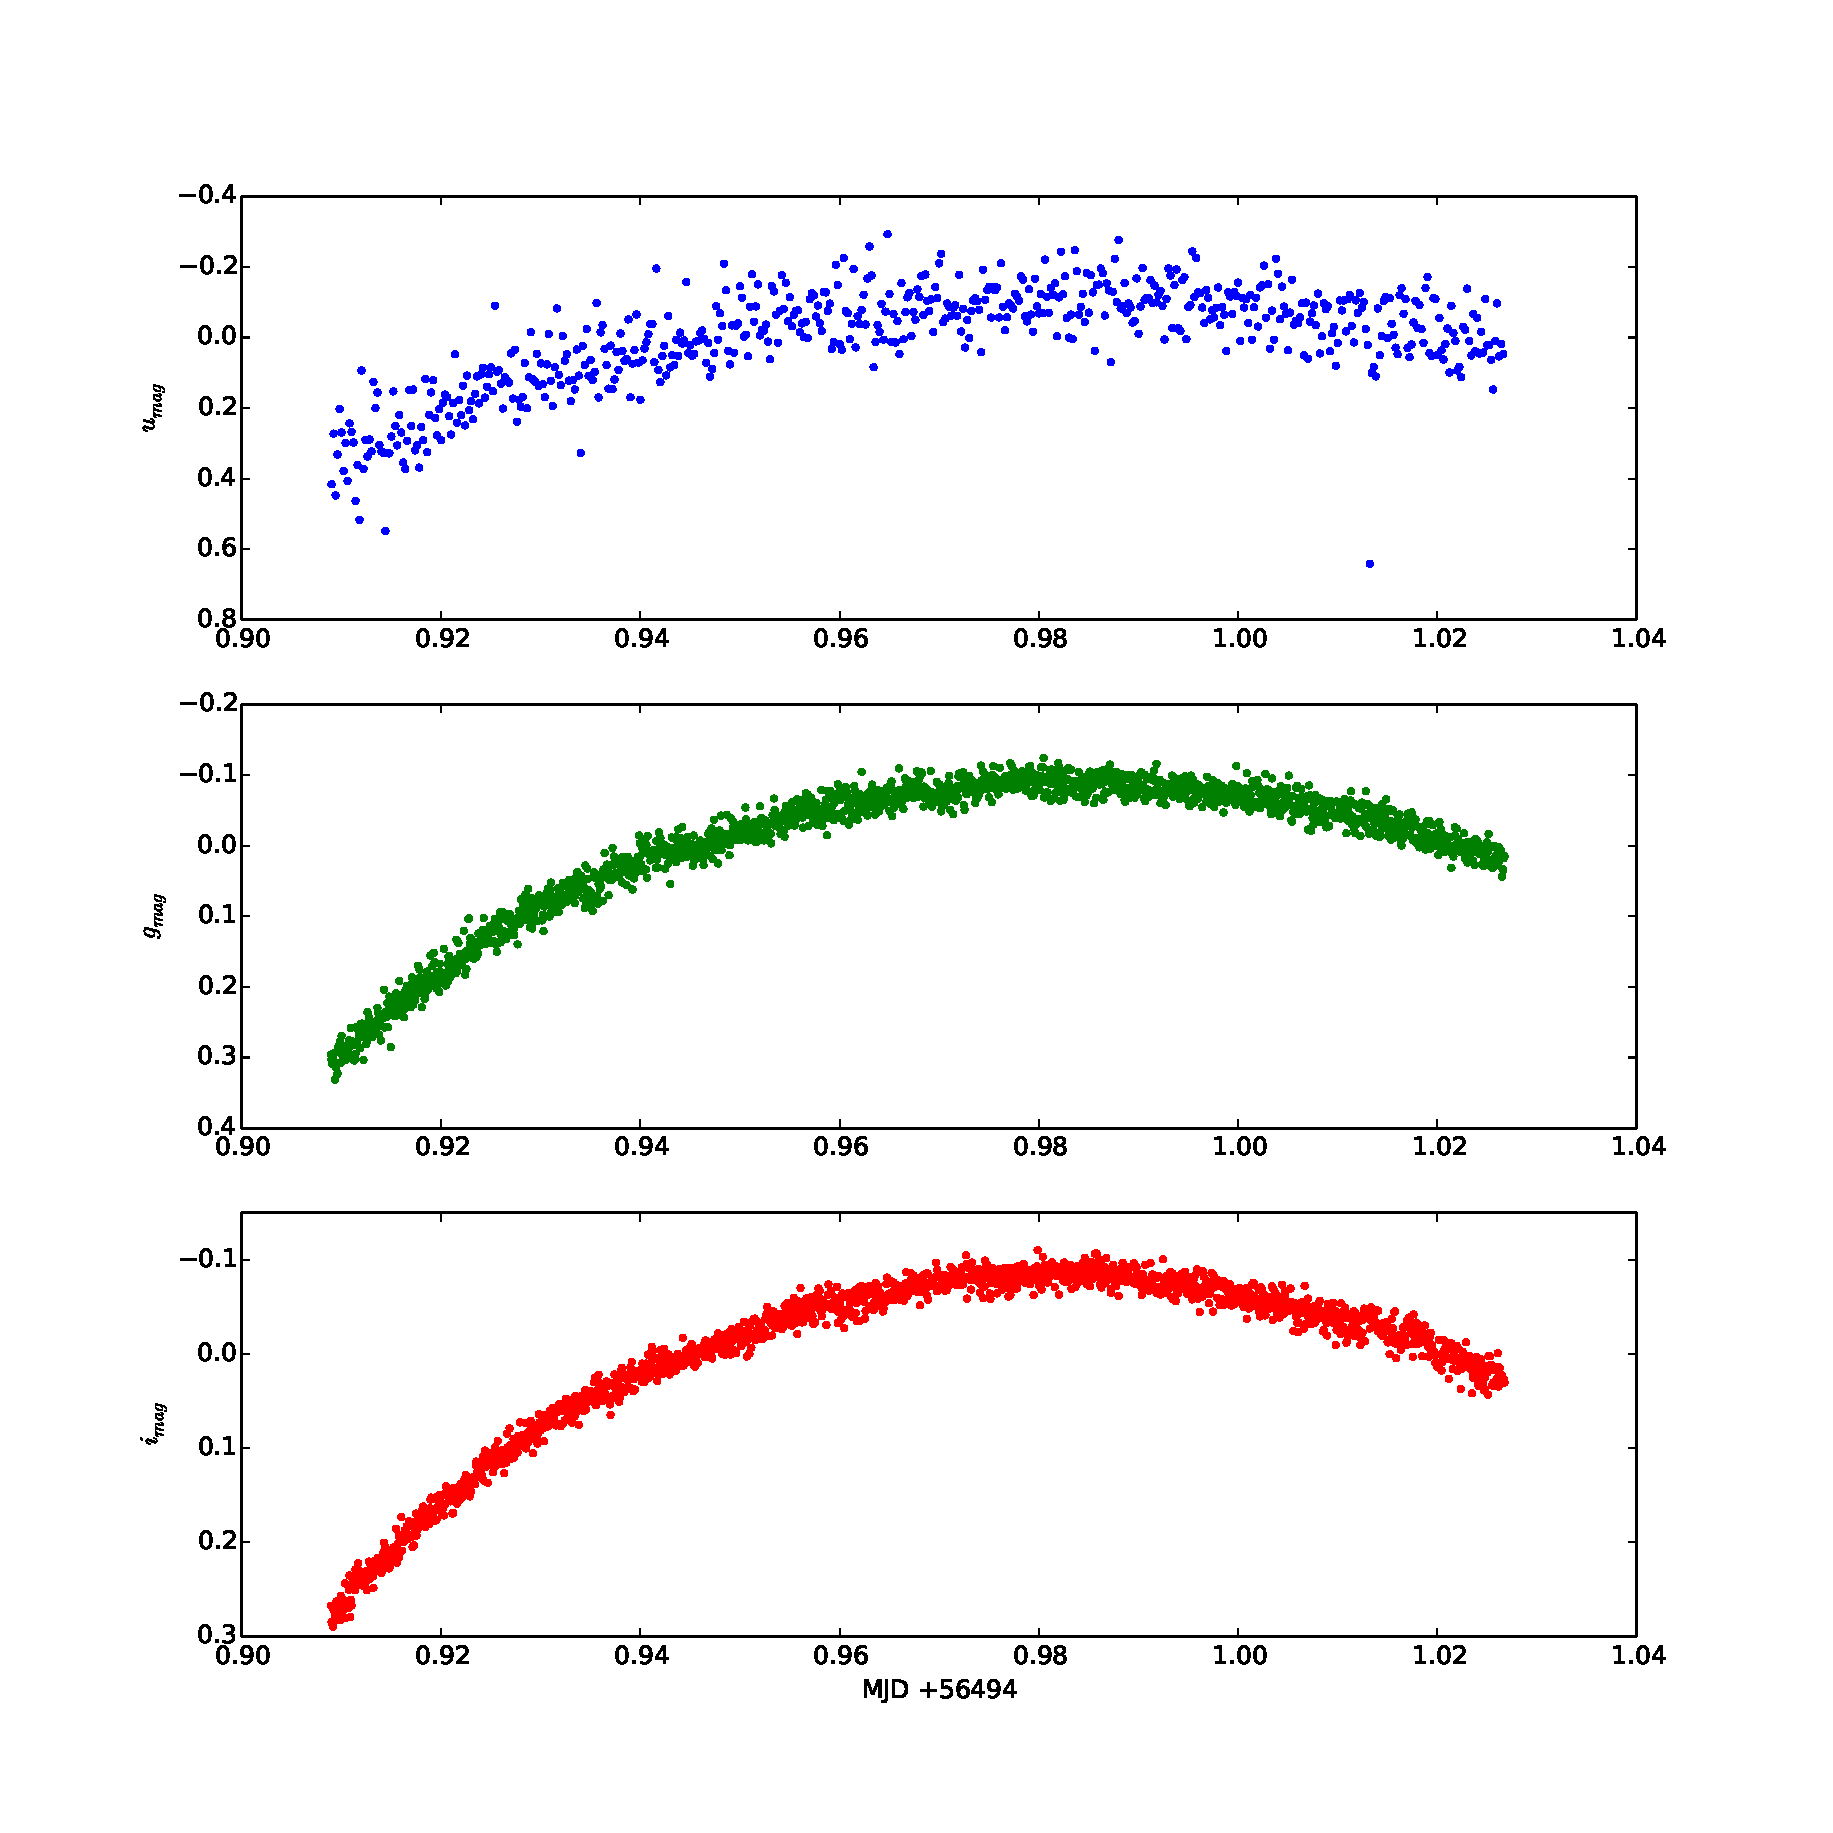
\includegraphics[width=120mm]{images/2013-07-21-run010-48_lightcurve.eps} \\
  Discussion of this object.

  \begin{tabular}{l l}
  Classification & W Uma contact binary \\
  ObjectID & 2013-07-21-run010-163 \\
  RA, DEC & 19:44:10.3, 40:18:08.1 (J2000) \\
  Run date & 2013-07-21 \\
  Pixel position & (417, 650) \\
  URL: & \small \url{http://deneb.astro.warwick.ac.uk/phrnaw/sitedev/2013-07-21/run010.html} \\
  Finding chart & 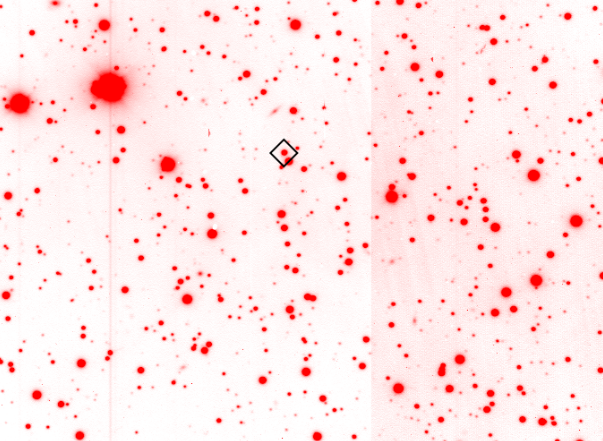
\includegraphics[width=60mm]{images/2013-07-21-run010-163.png} \\
  \end{tabular}
  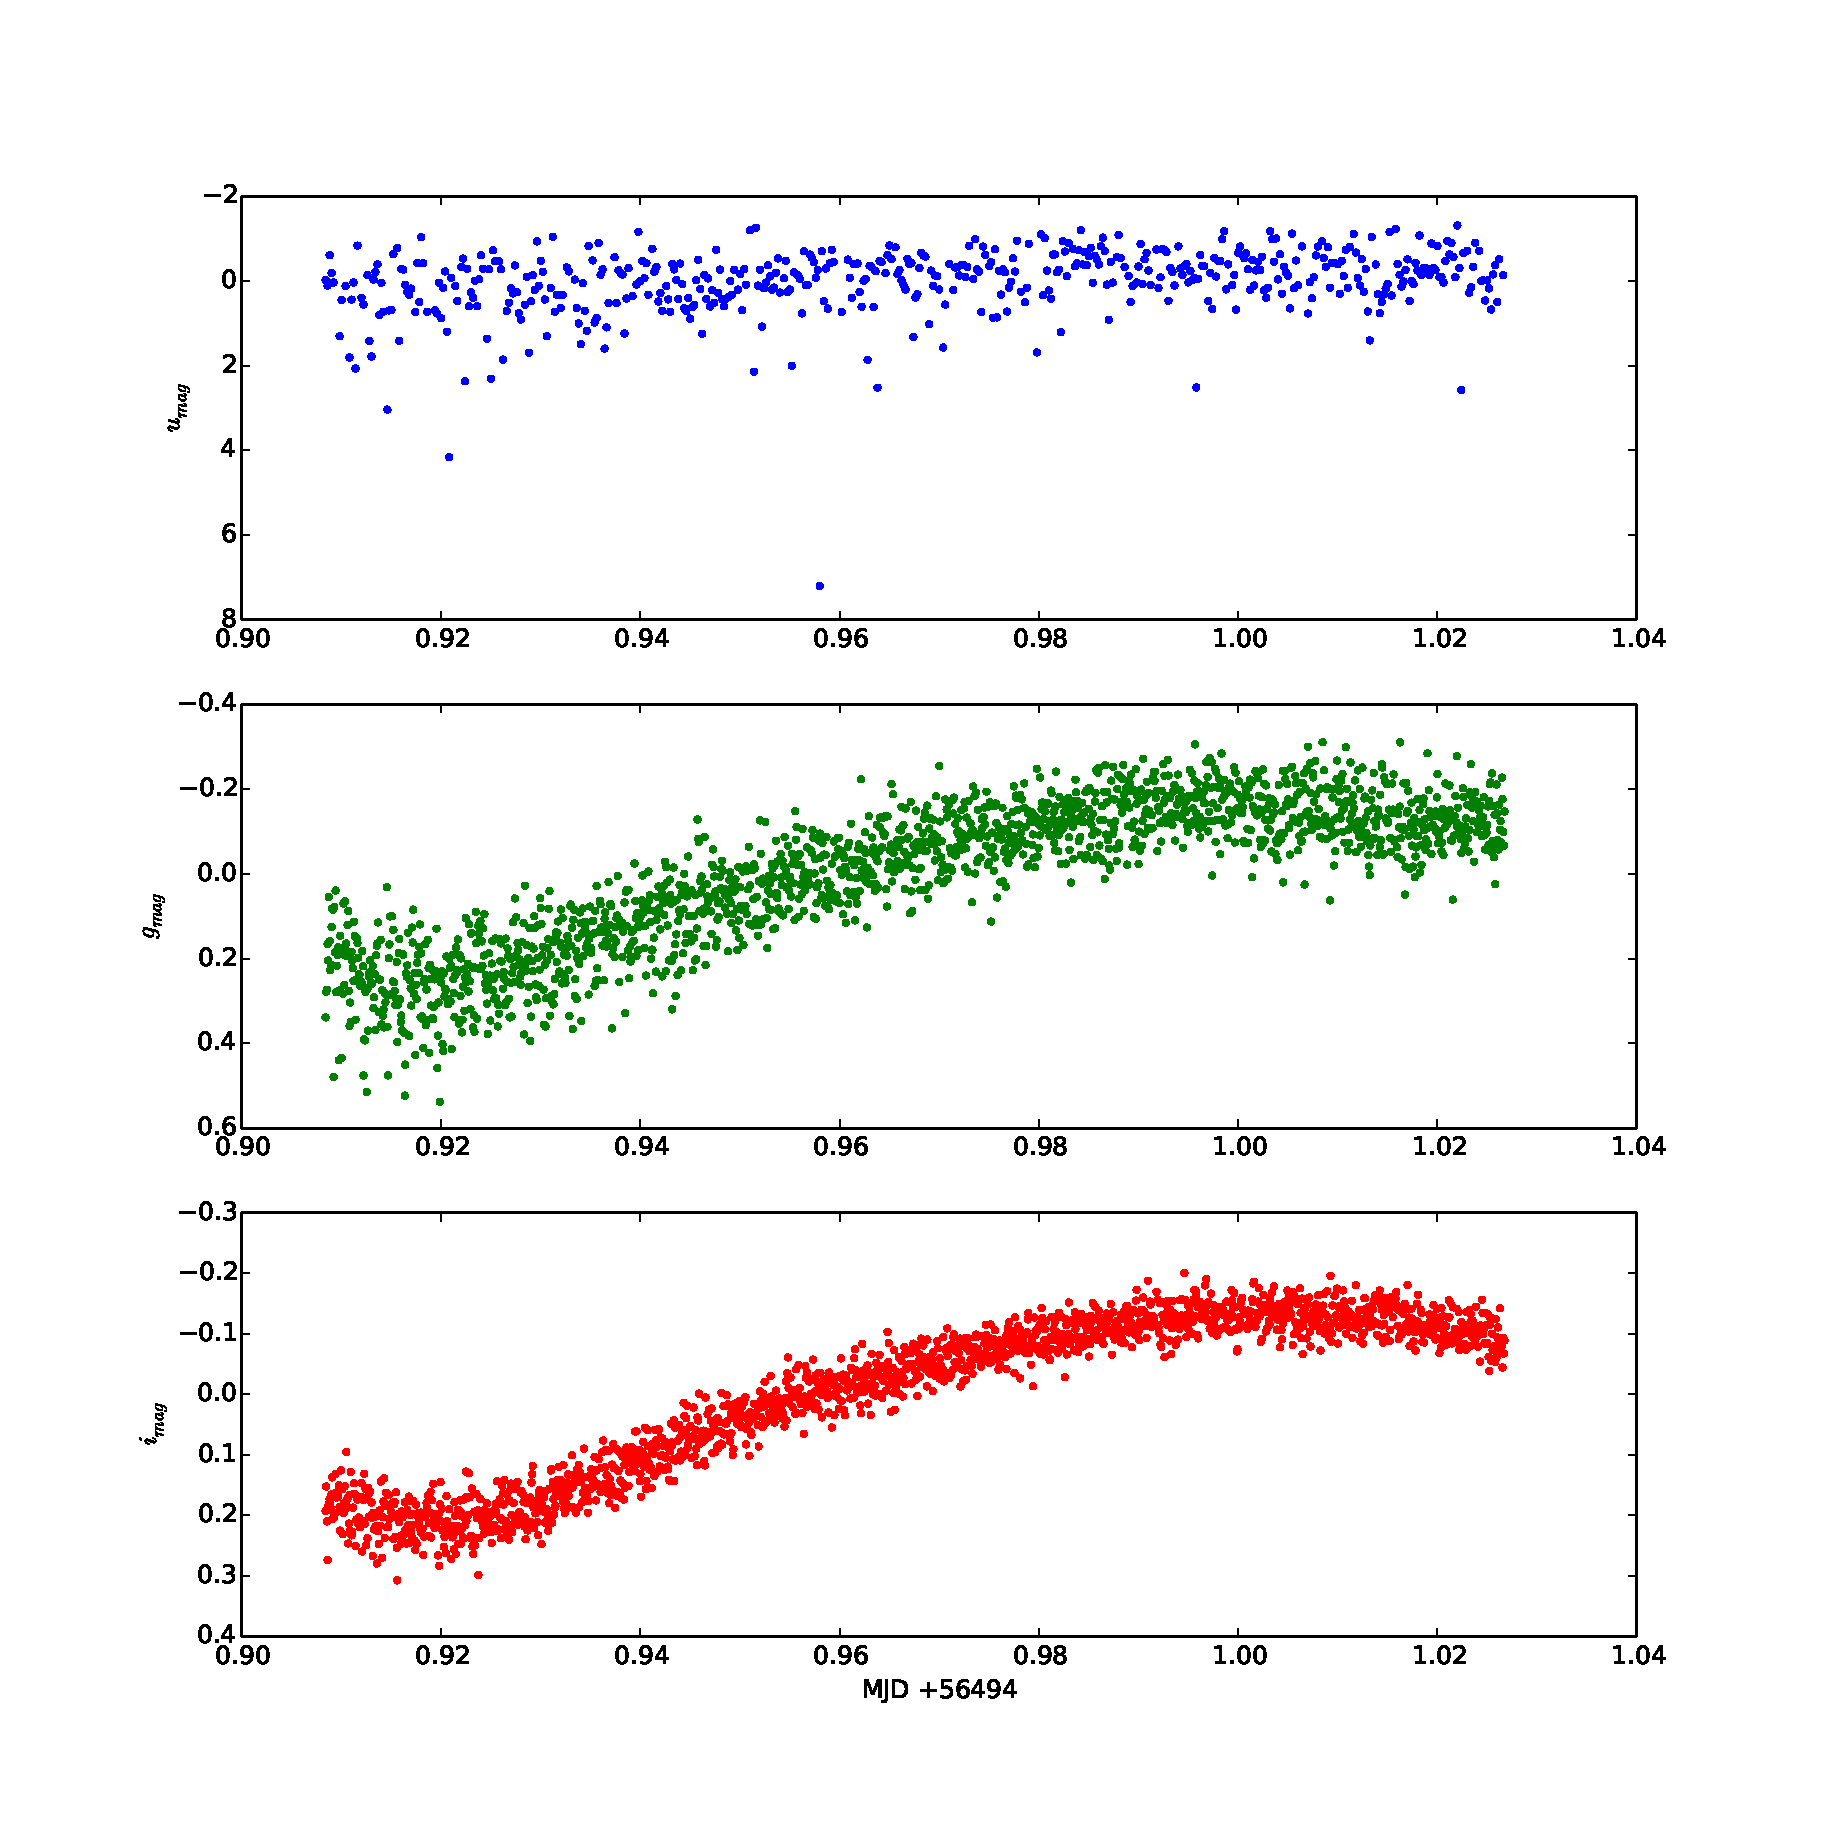
\includegraphics[width=120mm]{images/2013-07-21-run010-163_lightcurve.eps} \\
  Discussion of this object.

\begin{tabular}{l l}
  Classification & Eclipsing dwarf binary \\
  ObjectID & 2013-07-21-run011-162 \\
  Pixel position & (726, 341) \\
  RA, DEC & 19:54:02.6, 40:37:32.4 (J2000) \\
  URL: & \small \url{http://deneb.astro.warwick.ac.uk/phrnaw/sitedev/2013-07-21/run011.html} \\
  Finding chart & 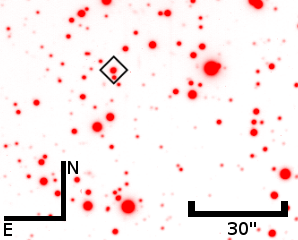
\includegraphics[width=60mm]{images/2013-07-21-run011-162.png} \\
  \end{tabular}
  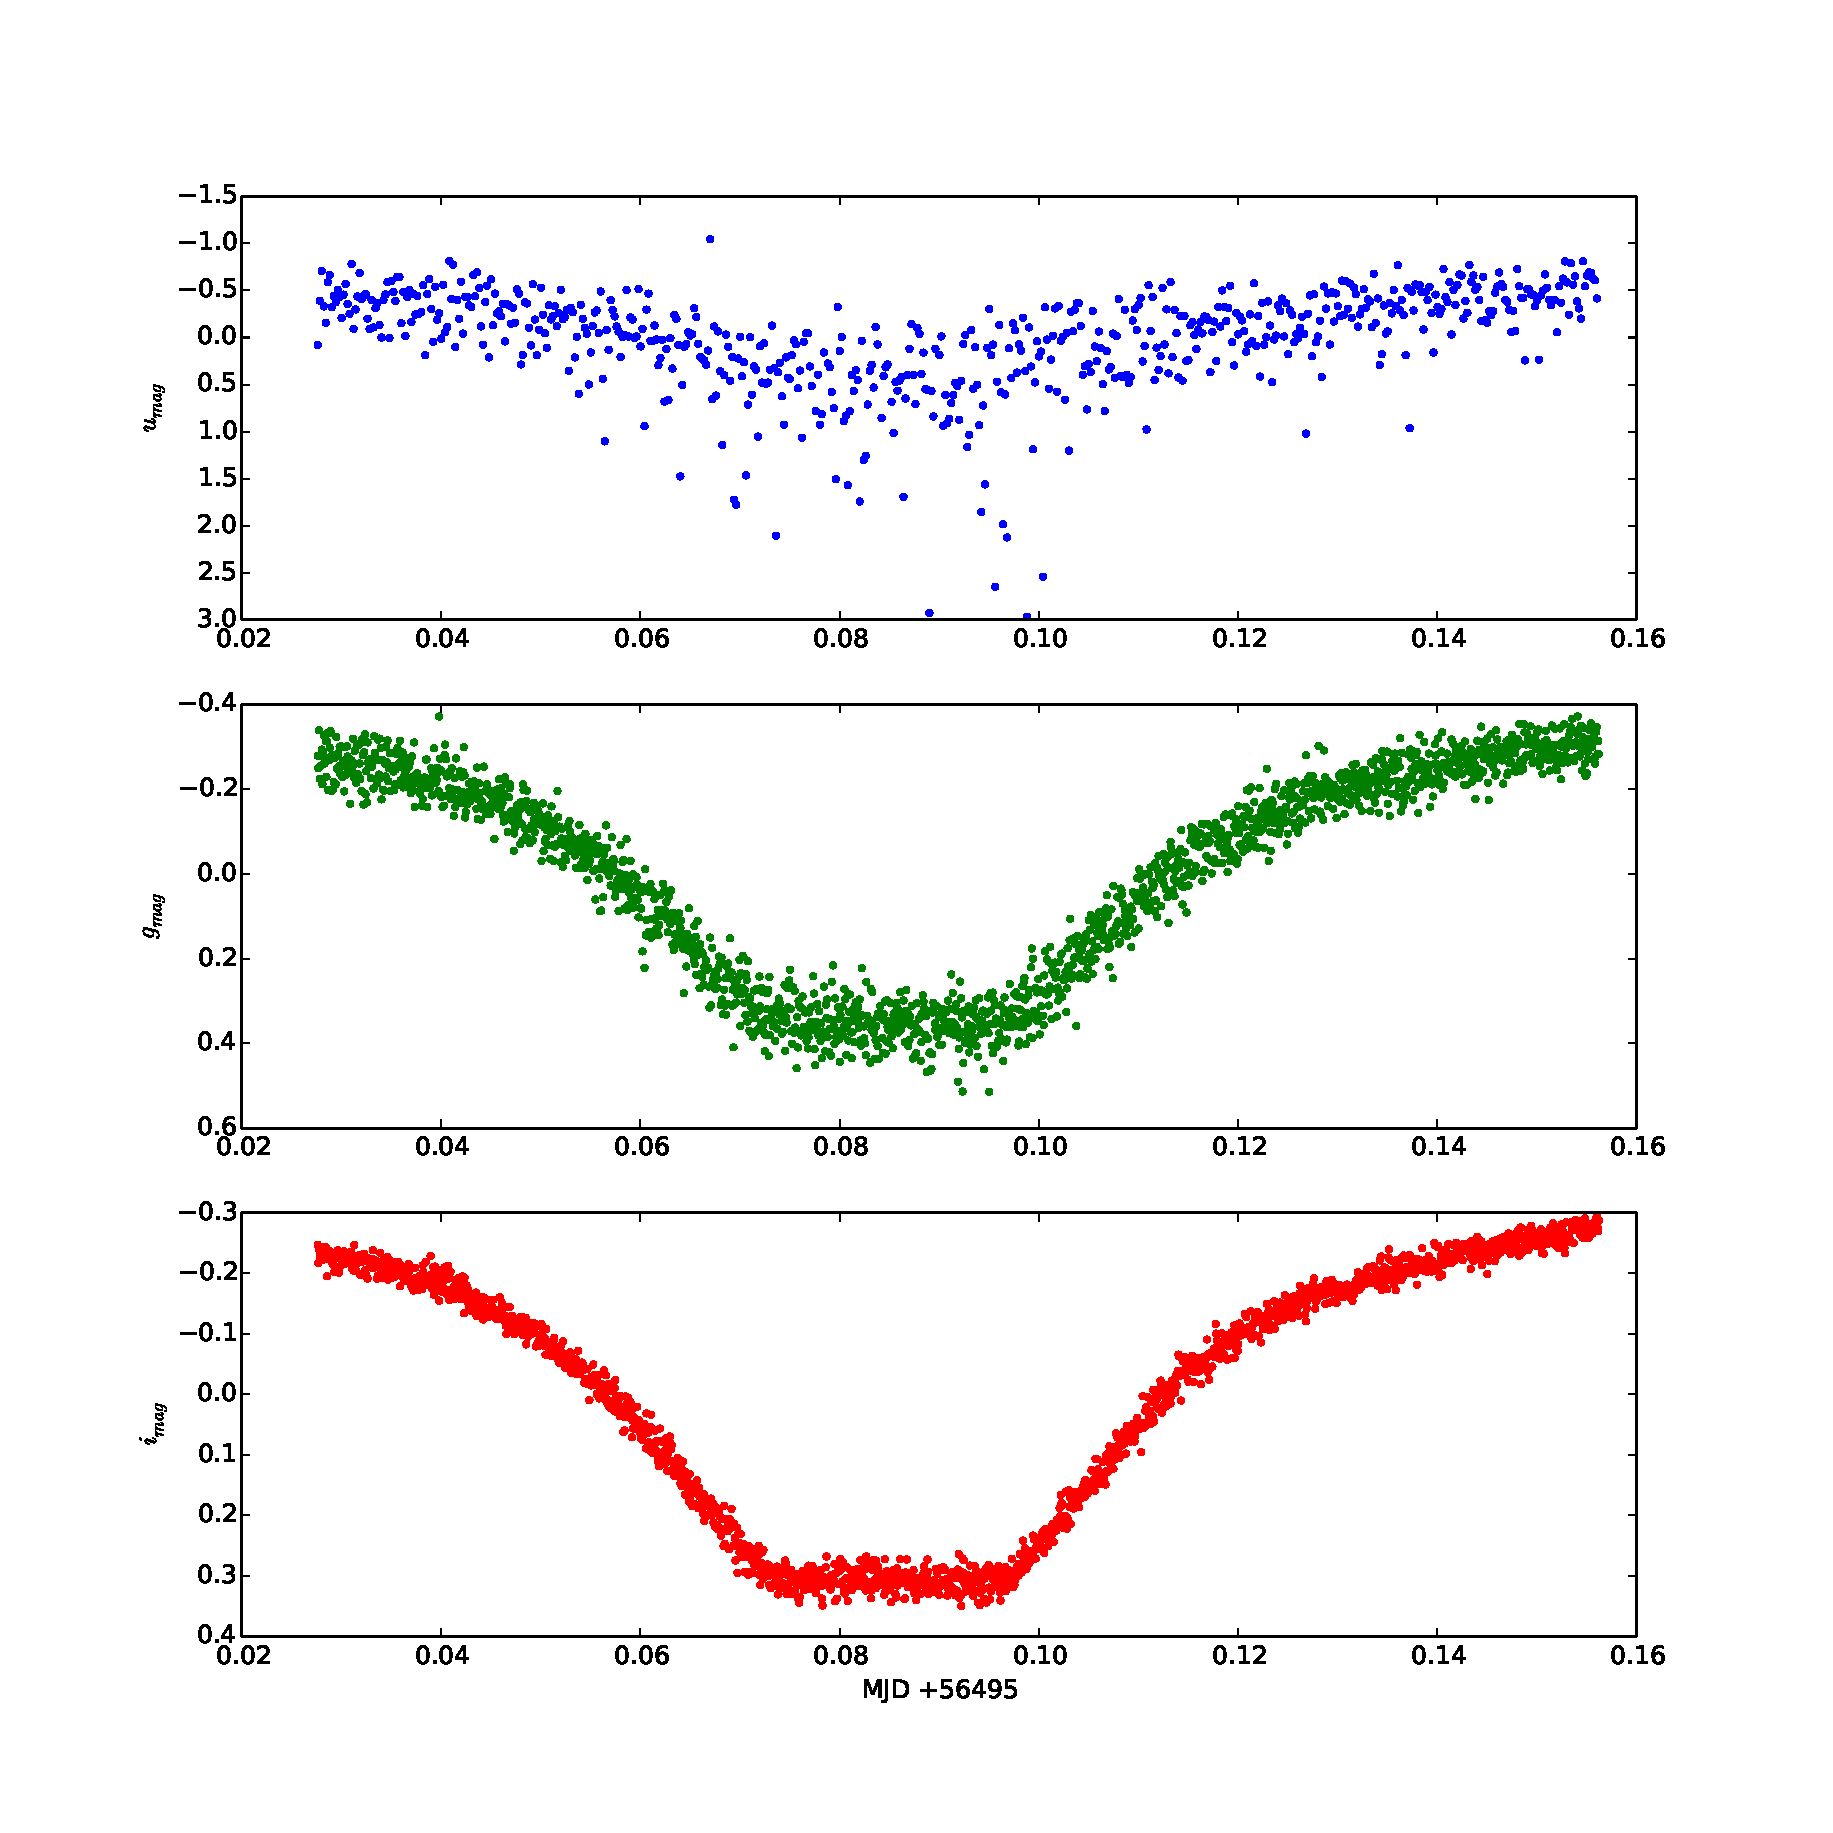
\includegraphics[width=120mm]{images/2013-07-21-run011-162_lightcurve.eps} \\
  Discussion of this object.

\subsection{Intrinsic variables}

  \begin{tabular}{l l}
  Classification & $\delta$ Scuti \\
  ObjectID & 2013-07-21-run010-23 \\
  Pixel position & (54, 362) \\
  RA, DEC & 19:44:17.53, 40:16:43.7 (J2000) \\
  URL: & \small \url{http://deneb.astro.warwick.ac.uk/phrnaw/sitedev/2013-07-21/run010.html} \\
  Finding chart & 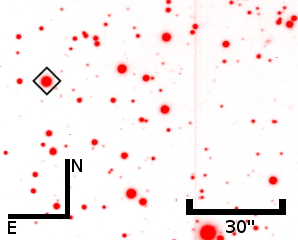
\includegraphics[width=60mm]{images/2013-07-21-run010-23.png} \\
  \end{tabular}
  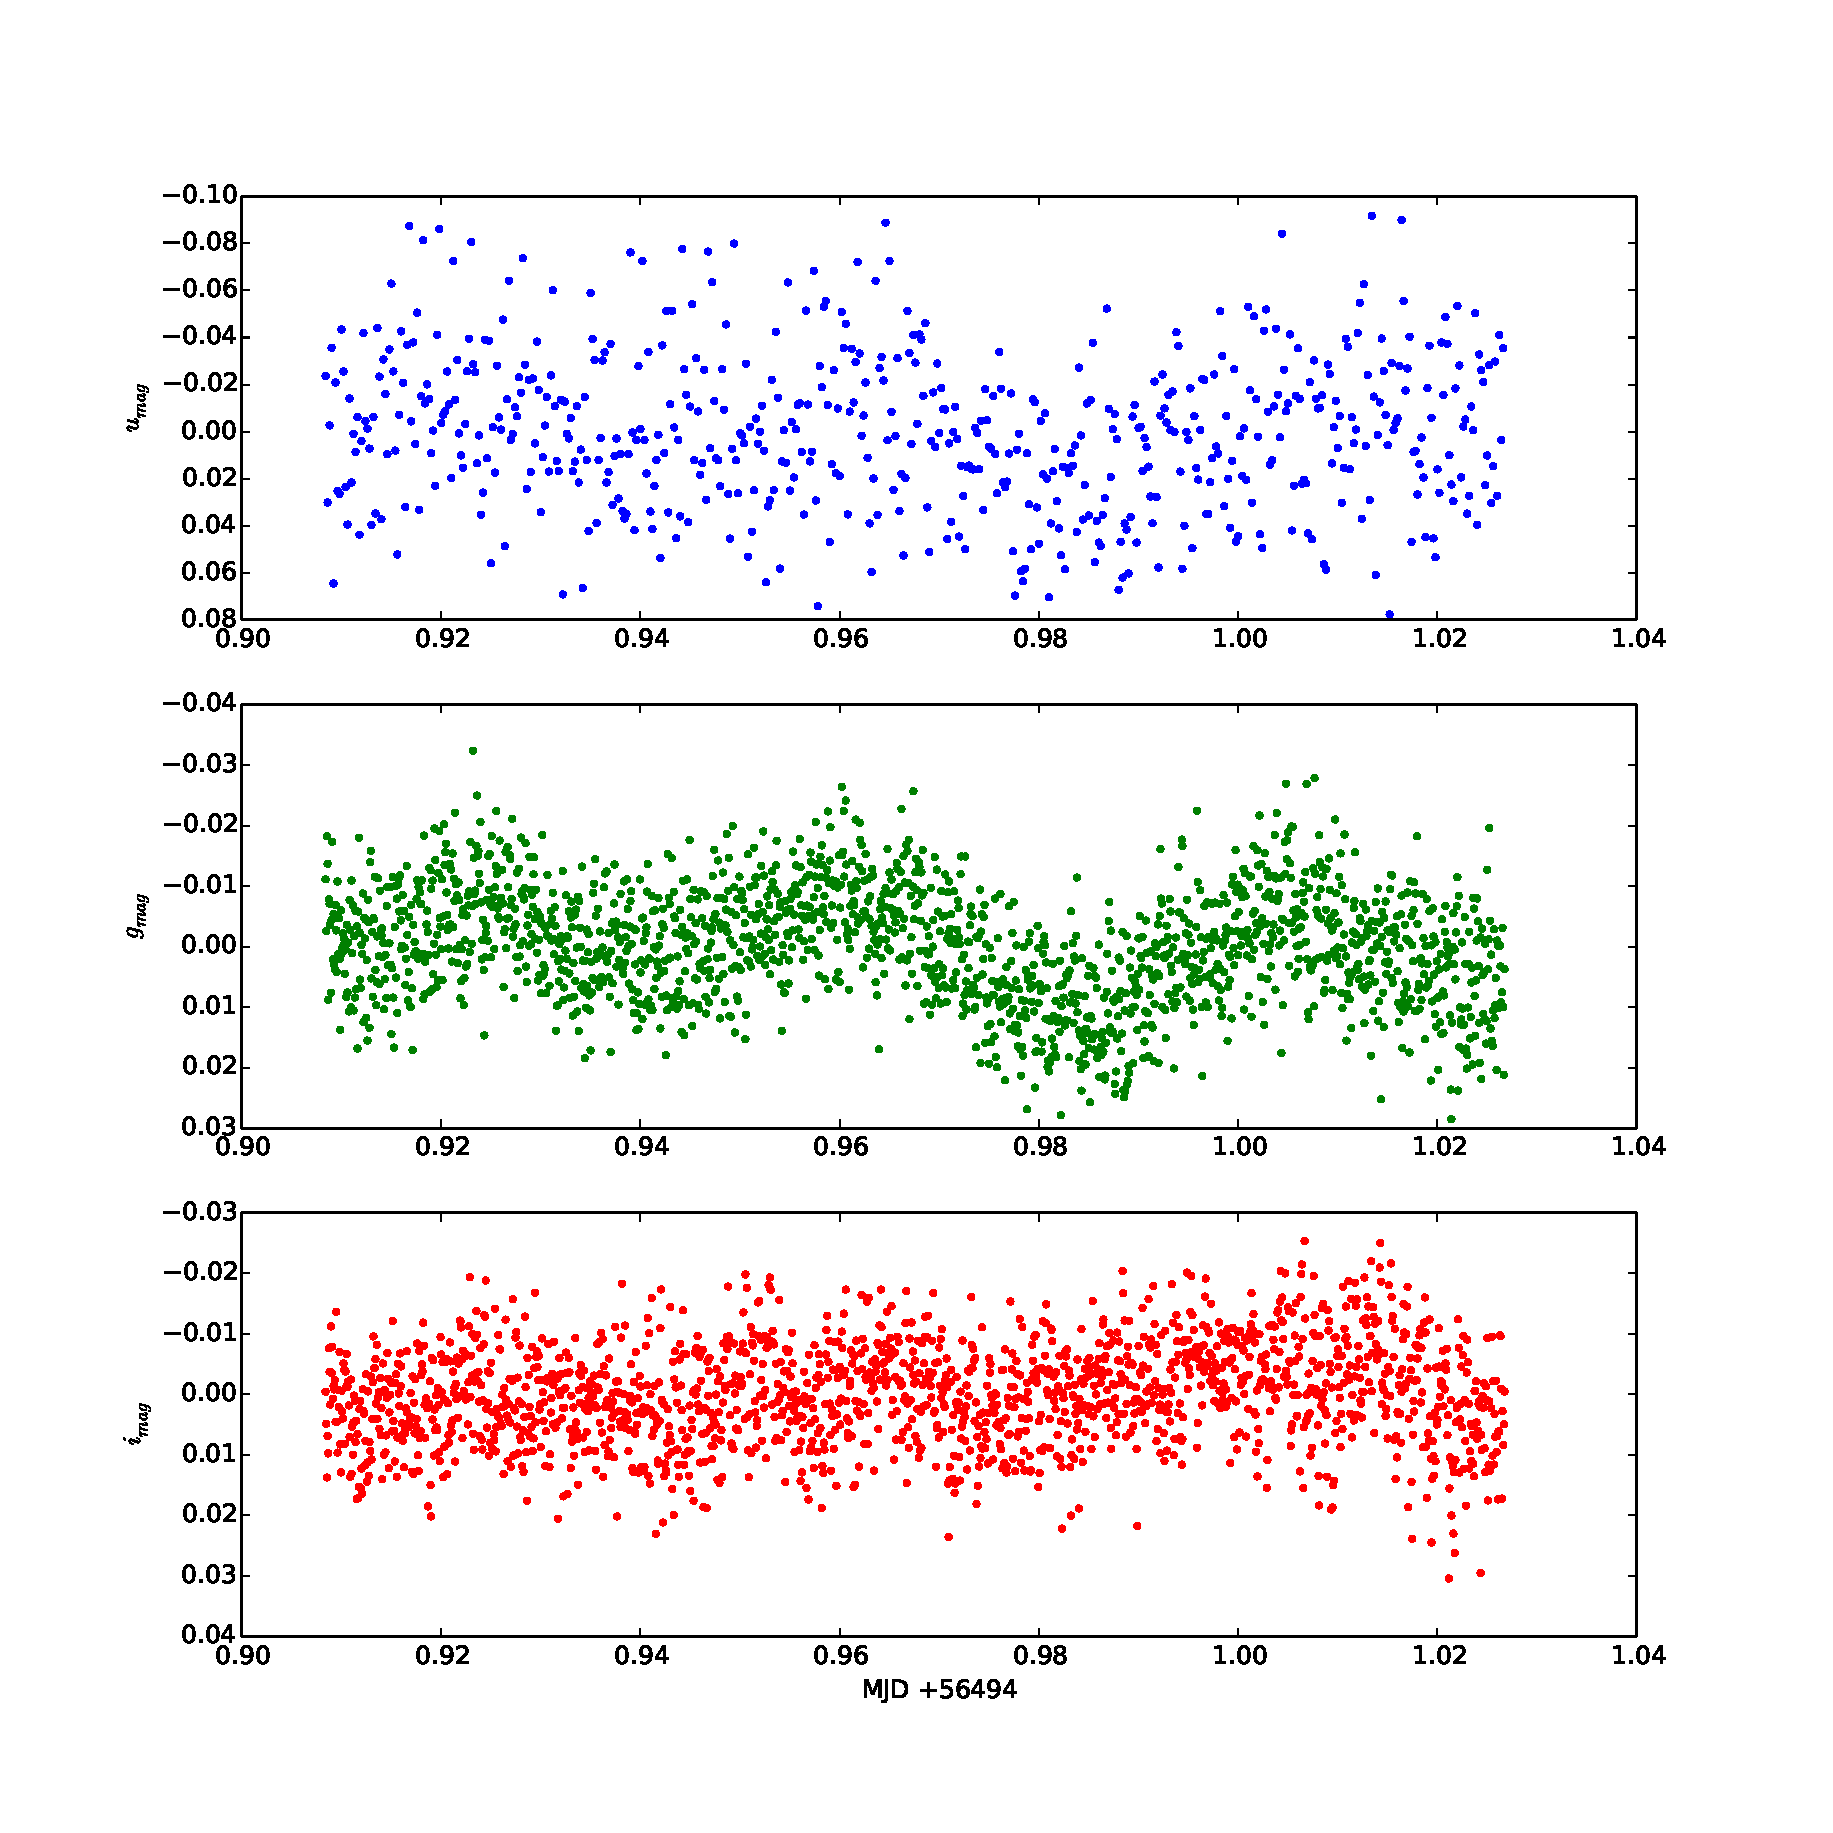
\includegraphics[width=120mm]{images/2013-07-21-run010-23_lightcurve.eps} \\
  Discussion of this object.


\subsection{Near Earth objects}

  \begin{tabular}{l l}
  Classification & Asteroid \\
  ObjectID & 2009-01-04-run024-61 \\
  Pixel position & start: (137, 422), end: (226, 447) \\
  Distance travelled & 92 pixels or 32" \\
  Field scale & 0.35"/pixel \\
  Duration of run & 3221s (53.7 minutes) \\
  Tangential angular velocity & 0.596"/minute or 35"/hour\\ 
  RA, DEC & ??? ??? (J2000) \\
  URL: & \small \url{http://deneb.astro.warwick.ac.uk/phrnaw/sitedev/2009-01-04/run024.html} \\
  Finding chart & 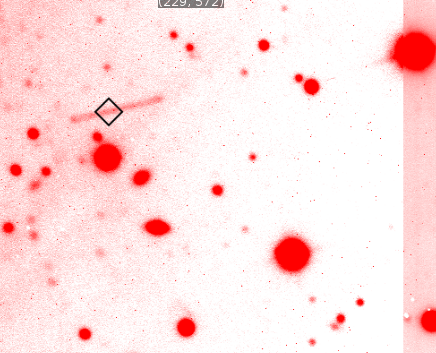
\includegraphics[width=60mm]{images/2009-01-04-run024-61.png} \\
  \end{tabular}
  Discussion of this object.
  